% BTVN_B8_1.tex - TDMXX22: TICH CO HUONG CUA HAI VECTO.
% Theo phong cach BTVN_B6.tex; hinh TikZ, khong can tep anh ngoai.
\documentclass[12pt,a4paper]{article}
\usepackage[left=15mm,right=15mm,top=14mm,bottom=18mm,footskip=9mm]{geometry}
\usepackage{iftex}
\ifPDFTeX
  \usepackage[T5]{fontenc}\usepackage[utf8]{inputenc}\usepackage{mathptmx}
\else
  \usepackage{fontspec}
  \IfFontExistsTF{Times New Roman}{\setmainfont{Times New Roman}}{%
    \IfFontExistsTF{Liberation Serif}{\setmainfont{Liberation Serif}}{\setmainfont{Latin Modern Roman}}}
\fi
\usepackage{amsmath,amssymb,fix-cm}
\usepackage{tikz}
\usetikzlibrary{arrows.meta}
\usepackage{tcolorbox,tabularx,fancyhdr,lastpage,needspace}
\definecolor{sectionpurple}{RGB}{155,42,143}
\definecolor{notebackground}{RGB}{229,240,245}
\definecolor{noteborder}{RGB}{255,55,55}
\definecolor{grblue}{RGB}{37,77,194}
\setlength{\parindent}{0pt}
\setlength{\parskip}{0pt}
\setlength{\headheight}{15pt}
\pagestyle{fancy}\fancyhf{}
\renewcommand{\headrulewidth}{0pt}\renewcommand{\footrulewidth}{0.4pt}
\fancyfoot[L]{\fontsize{8.5}{10}\selectfont Biên soạn: \textbf{Nguyễn Anh Dũng}}
\fancyfoot[R]{\fontsize{8.5}{10}\selectfont Trang \thepage/\pageref{LastPage} -- BTVN B8.1}
\newtcolorbox{notebox}{colback=notebackground,colframe=noteborder,
 boxrule=.65pt,arc=1.5pt,left=5pt,right=5pt,top=2pt,bottom=2pt,
 before skip=0pt,after skip=0pt}
\newcommand{\question}[2][TDM31]{%
  \par\noindent\textbf{\textcolor{sectionpurple}{Câu #2:} \textcolor{noteborder}{[#1]}}\enspace}
\newcommand{\answerlabel}[1]{\textbf{\textcolor{sectionpurple}{#1.}}}
\newcommand{\fourchoices}[4]{%
 \par\nobreak\vspace{1pt}\begin{tabular*}{\linewidth}{@{}l@{\extracolsep{\fill}}lll@{}}
 \answerlabel{A} #1 & \answerlabel{B} #2 & \answerlabel{C} #3 & \answerlabel{D} #4
 \end{tabular*}\par}
\newcommand{\twochoices}[4]{%
 \par\nobreak\vspace{1pt}\begin{tabularx}{\linewidth}{@{}>{\raggedright\arraybackslash}X>{\raggedright\arraybackslash}X@{}}
 \answerlabel{A} #1 & \answerlabel{B} #2 \\[1pt]
 \answerlabel{C} #3 & \answerlabel{D} #4
 \end{tabularx}\par}
\newcommand{\tfbox}[4]{%
\begin{notebox}\renewcommand{\arraystretch}{1.17}\setlength{\tabcolsep}{4pt}
\begin{tabularx}{\linewidth}{|>{\bfseries\color{sectionpurple}}c|>{\raggedright\arraybackslash}X|c|c|}
\hline\multicolumn{2}{|c|}{\textbf{\textcolor{sectionpurple}{Mệnh đề}}}&
\textbf{\textcolor{sectionpurple}{Đ}}&\textbf{\textcolor{sectionpurple}{S}}\\\hline
 a & #1 & $\bigcirc$ & $\bigcirc$ \\ \hline
 b & #2 & $\bigcirc$ & $\bigcirc$ \\ \hline
 c & #3 & $\bigcirc$ & $\bigcirc$ \\ \hline
 d & #4 & $\bigcirc$ & $\bigcirc$ \\ \hline
\end{tabularx}\end{notebox}}
\newcommand{\shortanswer}{%
 \par\nobreak\hfill
\begin{tikzpicture}[baseline=-.7ex]
 \node[draw=noteborder,fill=notebackground,line width=.6pt,rounded corners=1pt,
 minimum width=23mm,minimum height=5mm,inner sep=0pt] {};
 \end{tikzpicture}\par}
\newcommand{\examtitle}[2]{%
 \par\begin{center}\textbf{ĐỀ #1}\\[-1pt]\textbf{#2}\\[-1pt]
 {\fontsize{10.5}{12}\selectfont\itshape Form đề chuẩn bám sát BGD2026 -- Thời gian làm bài \textbf{90 phút}}\end{center}\vspace{-7pt}}
\newcommand{\partone}[1]{\par\textbf{Phần I. Câu trắc nghiệm nhiều phương án lựa chọn.} Thí sinh trả lời từ câu 1 đến câu #1. Mỗi câu chỉ chọn một phương án.\par}
\newcommand{\parttwo}[2]{\par\addvspace{2pt}\textbf{Phần II. Câu trắc nghiệm đúng sai.} Thí sinh trả lời từ câu #1 đến câu #2, trong mỗi ý a), b), c), d) chọn đúng hoặc sai.\par}
\newcommand{\partthree}[2]{\par\addvspace{2pt}\textbf{Phần III. Câu trắc nghiệm trả lời ngắn.} Thí sinh trả lời từ câu #1 đến câu #2.\par}
\newcommand{\finishExam}{\par\vspace{3pt}{\centering\textbf{\textcolor{sectionpurple}{--- Hết ---}}\par}}
% Hinh lap phuong va so do can cau duoc ve bang TikZ theo PDF (TDMXX20).
% Hinh TikZ doc lap, khong can tai tep hinh ben ngoai.
\newcommand{\figbox}[1]{%
\begin{notebox}\centering
\begin{tikzpicture}[x=.43cm,y=.43cm,>=Stealth,every node/.style={font=\fontsize{10}{11}\selectfont}]
 #1
\end{tikzpicture}\end{notebox}}
\newcommand{\axes}[4]{%
 \draw[thin,-{Stealth[length=4pt]}] (#1,0)--(#2,0) node[below] {$x$};
 \draw[thin,-{Stealth[length=4pt]}] (0,#3)--(0,#4) node[right] {$y$};
 \node[below left] at (0,0) {$O$};}
\newcommand{\dotat}[2]{\fill (#1,#2) circle (1.3pt);}
\newcommand{\vguide}[2]{\draw[thin,densely dashed] (#1,0)--(#1,#2);\dotat{#1}{0}\dotat{#1}{#2}}

\newcommand{\cubefig}{%
\begin{notebox}\centering
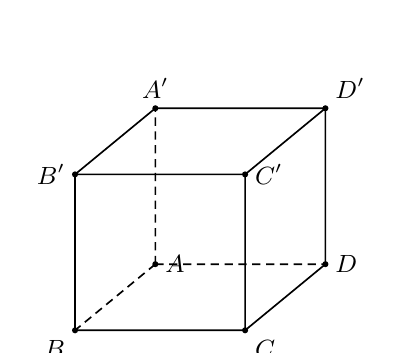
\begin{tikzpicture}[x=.60cm,y=.60cm,line width=.6pt,every node/.style={font=\small}]
 \coordinate (A) at (1.7,1.4); \coordinate (B) at (0,0);
 \coordinate (C) at (3.6,0); \coordinate (D) at (5.3,1.4);
 \coordinate (Ap) at (1.7,4.7); \coordinate (Bp) at (0,3.3);
 \coordinate (Cp) at (3.6,3.3); \coordinate (Dp) at (5.3,4.7);
 \draw[densely dashed] (A)--(B) (A)--(D) (A)--(Ap);
 \draw (B)--(C)--(D)--(Dp)--(Ap)--(Bp)--(B)
       (Bp)--(Cp)--(Dp) (Cp)--(C);
 \foreach \p in {A,B,C,D,Ap,Bp,Cp,Dp}{\fill (\p) circle (1.1pt);}
 \node[right] at (A) {$A$}; \node[below left] at (B) {$B$};
 \node[below right] at (C) {$C$}; \node[right] at (D) {$D$};
 \node[above] at (Ap) {$A'$}; \node[left] at (Bp) {$B'$};
 \node[right] at (Cp) {$C'$}; \node[above right] at (Dp) {$D'$};
\end{tikzpicture}\end{notebox}}
\newcommand{\cranefig}{%
\begin{notebox}\centering
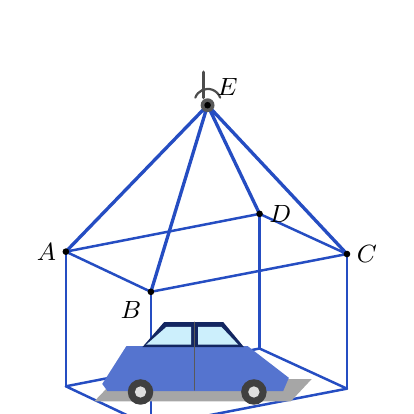
\begin{tikzpicture}[x=.60cm,y=.60cm,line join=round,line cap=round,every node/.style={font=\small}]
 \coordinate (E) at (0,6.15);
 \coordinate (A) at (-3,3.05); \coordinate (B) at (-1.20,2.20);
 \coordinate (C) at (2.95,3.00); \coordinate (D) at (1.10,3.85);
 \coordinate (Ab) at (-3,.20); \coordinate (Bb) at (-1.20,-.65);
 \coordinate (Cb) at (2.95,.15); \coordinate (Db) at (1.10,1.00);
 \draw[line width=1.2pt,grblue] (E)--(A) (E)--(B) (E)--(C) (E)--(D);
 \draw[grblue,line width=.9pt] (A)--(B)--(C)--(D)--cycle;
 \draw[grblue,line width=.9pt] (A)--(Ab) (B)--(Bb) (C)--(Cb) (D)--(Db);
 \draw[grblue,line width=.9pt] (Ab)--(Bb)--(Cb)--(Db)--cycle;
 \draw[very thick,gray!60!black] (-.08,6.85)--(-.08,6.31);
 \fill[gray!70!black] (E) circle (2.5pt);
 \draw[thick,gray!60!black] (-.26,6.31) arc[start angle=160,end angle=20,radius=.28];
 \fill[black!35] (-2.40,-.12)--(1.76,-.12)--(2.20,.35)--(-1.95,.35)--cycle;
 \fill[grblue!78] (-2.23,.25)--(-1.72,1.05)--(.85,1.05)--(1.72,.38)--(1.60,.10)--(-2.12,.10)--cycle;
 \fill[grblue!50!black] (-1.38,1.03)--(-.92,1.56)--(.33,1.56)--(.77,1.03)--cycle;
 \fill[cyan!20] (-1.30,1.08)--(-.87,1.46)--(-.35,1.46)--(-.35,1.08)--cycle;
 \fill[cyan!20] (-.20,1.08)--(-.20,1.46)--(.29,1.46)--(.65,1.08)--cycle;
 \draw[black!65,thin] (-.27,.12)--(-.27,1.56);
 \fill[black!75] (-1.42,.08) circle (.27) (.98,.08) circle (.27);
 \fill[gray!25] (-1.42,.08) circle (.12) (.98,.08) circle (.12);
 \foreach \p/\where in {E/above right,A/left,B/below left,C/right,D/right}
    {\fill (\p) circle (1.2pt);\node[\where] at (\p) {$\p$};}
\end{tikzpicture}\end{notebox}}


\begin{document}
\fontsize{11.5}{14}\selectfont
\examtitle{TDMXX22}{TÍCH CÓ HƯỚNG CỦA HAI VECTƠ}
\partone{12}

\question[TDM21]{1} Trong không gian $Oxyz$, cho hai vectơ $\vec{u}=(2;-1;3)$ và $\vec{v}=(2;2;1)$. Tích có hướng của $\vec{u}$ và $\vec{v}$ là
\fourchoices{$(7;-4;-6)$.}{$(-7;4;6)$.}{$(2;-3;1)$.}{$(5;0;0)$.}

\question[TDM21]{2} Trong không gian $Oxyz$, cho hai vectơ $\vec{u}=(1;3;2)$ và $\vec{v}=(4;0;-1)$. Vectơ $[\vec{u},\vec{v}]$ có tọa độ là
\fourchoices{$(-3;9;-12)$.}{$(4;-1;5)$.}{$(11;0;4)$.}{$(-9;-3;15)$.}

\question[TDM21]{3} Trong không gian $Oxyz$, nhận xét \textbf{sai} là
\fourchoices{$[\vec{i},\vec{j}]=\vec{k}$.}{$[\vec{j},\vec{k}]=\vec{i}$.}{$[\vec{i},\vec{k}]=\vec{j}$.}{$[\vec{k},\vec{j}]+\vec{i}=\vec{0}$.}

\question[TDM21]{4} Trong không gian $Oxyz$, cho hai vectơ $\vec{u}$ và $\vec{v}$. Gọi vectơ $\vec{a}$ là tích có hướng của vectơ $\vec{u}$ với vectơ $\vec{v}$. Nhận xét \textbf{sai} là
\fourchoices{$\vec{a}\perp\vec{u}$.}{$\vec{a}\perp\vec{v}$.}{$\vec{a}=-[\vec{v},\vec{u}]$.}{$\vec{a}=-[\vec{u},\vec{v}]$.}

\question[TDM22]{5} Trong không gian $Oxyz$, cho hai vectơ $\vec{u}$ và $\vec{v}$. Biết rằng $[\vec{u},\vec{v}]=\vec{0}$. Nhận xét nào dưới đây chắc chắn \textbf{sai}?
\fourchoices{$\vec{u}=\vec{0}$.}{$\vec{v}=\vec{0}$.}{$|\vec{u}\cdot\vec{v}|<|\vec{u}|\,|\vec{v}|$.}{$\vec{u}\parallel\vec{v}$.}

\question[TDM31]{6} Trong không gian $Oxyz$, cho ba điểm có tọa độ là $A(3;-1;1)$, $B(4;-2;0)$, $C(3;-2;-2)$. Vectơ nào dưới đây là VTPT của mặt phẳng $(ABC)$?
\fourchoices{$(2;3;-1)$.}{$(3;0;1)$.}{$(-1;2;-3)$.}{$(4;2;-3)$.}

\question[TDM31]{7} Trong không gian $Oxyz$, cho bốn điểm $A,B,C,D$ đồng phẳng. Trong các nhận xét dưới đây, nhận xét có thể \textbf{sai} là
\fourchoices{$[\overrightarrow{AB},\overrightarrow{AC}]\cdot\overrightarrow{AD}=0$.}{$[\overrightarrow{AB},\overrightarrow{AD}]\cdot\overrightarrow{AC}=0$.}{$[\overrightarrow{BA},\overrightarrow{BC}]\cdot\overrightarrow{BD}=0$.}{$[\overrightarrow{CA},\overrightarrow{CB}]=\vec{0}$.}

\question[TDM31]{8} Trong không gian $Oxyz$, cho bốn điểm $A(0;3;0)$, $B(-2;1;0)$, $C(1;0;3)$, $D(0;0;m)$ đồng phẳng. Giá trị của tham số $m$ nằm trong khoảng nào dưới đây?
\fourchoices{$\left(\dfrac52;4\right)$.}{$(-2;0)$.}{$\left(2;\dfrac52\right)$.}{$(0;2)$.}

\question[TDM41]{9} Trong không gian $Oxyz$, cho bốn điểm $A(2;-1;1)$, $B(1;-2;2)$, $C(1;2;-3)$, $D(3;0;1)$. Hãy xác định \textbf{cosin} góc tạo bởi hai mặt phẳng $(BCD)$ và $(ABC)$?
\fourchoices{$\dfrac4{\sqrt{21}}$.}{$\dfrac{22}{5\sqrt{21}}$.}{$\dfrac3{\sqrt{26}}$.}{$\dfrac1{\sqrt3}$.}

\question[TDM41]{10} Trong không gian $Oxyz$, cho $5$ điểm $A(2;0;0)$, $B(2;2;1)$, $C(1;-1;2)$, $D(0;3;1)$, $E(3;-1;3)$. Hãy xác định \textbf{cosin} góc tạo bởi đường thẳng $AB$ và mặt phẳng $(CDE)$?
\fourchoices{$\dfrac{2\sqrt5}9$.}{$\dfrac{\sqrt3}6$.}{$\dfrac{\sqrt{61}}9$.}{$\dfrac{\sqrt2}4$.}

\question[TDM32]{11} Trong không gian $Oxyz$, cho ba điểm $A(1;0;-2)$, $B(0;1;2)$, $C(4;-1;0)$. Diện tích tam giác $ABC$ bằng
\fourchoices{$2\sqrt{59}$.}{$\sqrt{59}$.}{$\dfrac{\sqrt{59}}2$.}{$4\sqrt{59}$.}

\question[TDM32]{12} Trong không gian $Oxyz$, cho bốn điểm $A(2;1;1)$, $B(-2;2;1)$, $C(0;3;1)$, $D(3;0;0)$. Thể tích hình tứ diện $ABCD$ bằng
\fourchoices{$2$.}{$3$.}{$1$.}{$\dfrac16$.}

\parttwo{13}{16}
\question[TDM22]{13} Trong không gian $Oxyz$, cho hai vectơ $\vec{u}$, $\vec{v}$ và số thực $k$. Mệnh đề nào sau đây là \textbf{đúng hay sai}?
\tfbox{$[\vec{u},\vec{v}]=-[\vec{v},\vec{u}]$.}
{$[\vec{u},\vec{v}]=\vec{0}\Leftrightarrow\vec{u},\vec{v}$ cùng phương.}
{$\bigl([\vec{u},\vec{v}]\cdot\vec{u}\bigr)^2+\bigl([\vec{u},\vec{v}]\cdot\vec{v}\bigr)^2=0$.}
{$[k\vec{u},\vec{v}]=|k|[\vec{u},\vec{v}]$.}

\question[TDM22]{14} Trong không gian $Oxyz$, cho ba điểm phân biệt $A(1;0;0)$, $B(2;0;0)$, $C(0;0;4)$. Mệnh đề nào sau đây là \textbf{đúng hay sai}?
\tfbox{Vectơ $[\overrightarrow{AB},\overrightarrow{AC}]$ là một vectơ pháp tuyến của mặt phẳng $(ABC)$.}
{Hai vectơ $[\overrightarrow{AB},\overrightarrow{AC}]$ và $[\overrightarrow{BA},\overrightarrow{BC}]$ cùng phương.}
{Hai vectơ $[\overrightarrow{AB},\overrightarrow{AC}]$ và $[\overrightarrow{CB},\overrightarrow{CA}]$ không cùng phương.}
{Ba vectơ $[\overrightarrow{AB},\overrightarrow{AC}]$, $[\overrightarrow{BC},\overrightarrow{BA}]$, $[\overrightarrow{CA},\overrightarrow{CB}]$ đôi một bằng nhau.}

\question[TDM22_32]{15} Trong không gian $Oxyz$, cho ba điểm $A(1;0;0)$, $B(0;2;3)$, $C(1;0;-1)$. Mệnh đề nào sau đây là \textbf{đúng hay sai}?
\tfbox{Vectơ $[\overrightarrow{AB},\overrightarrow{AC}]=(-2;-1;0)$ là một vectơ pháp tuyến của mặt phẳng $(ABC)$.}
{$\cos\bigl([\overrightarrow{AB},\overrightarrow{AC}],\overrightarrow{BC}\bigr)=0$.}
{Nếu $\varphi_1$ là góc giữa hai mặt phẳng $(ABC)$ và $(OAB)$ thì $\cos\varphi_1=\dfrac12$.}
{Nếu $\varphi_2$ là góc giữa đường thẳng $OA$ và mặt phẳng $(ABC)$ thì $\cos\varphi_2=\dfrac45$.}

\question[TDM32]{16} Trong không gian $Oxyz$, cho bốn điểm $A(2;-2;0)$, $B(3;0;2)$, $C(-1;1;2)$, $D(2;1;3)$. Mệnh đề nào sau đây là \textbf{đúng hay sai}?
\tfbox{Diện tích tam giác $ABC$ bằng $\sqrt{149}$.}
{Thể tích tứ diện $ABCD$ bằng $1$.}
{$d(D,(ABC))=\dfrac3{\sqrt{149}}$.}
{$d(AB,CD)=\dfrac3{\sqrt{65}}$.}

\partthree{17}{22}
\question[TDM32]{17} Trong không gian $Oxyz$, cho hình bình hành $ABCD$ có tọa độ ba đỉnh $B(2;0;0)$, $C(0;1;3)$, $D(5;1;0)$. Hãy xác định diện tích hình bình hành $ABCD$? (Làm tròn kết quả đến hàng phần mười)
\shortanswer

\question[TDM32]{18} Trong không gian $Oxyz$, cho hình hộp $ABCD.A'B'C'D'$ có tọa độ bốn đỉnh $A(0;2;0)$, $B(1;0;0)$, $C(0;0;-3)$, $A'(1;0;-2)$. Thể tích hình hộp $ABCD.A'B'C'D'$ bằng
\shortanswer

\question[TDM32]{19} Trong không gian $Oxyz$, cho hình chóp $S.ABCD$ có đáy là hình bình hành và có tọa độ các điểm là $S(3;0;1)$, $A(2;0;0)$, $B(0;1;0)$, $C(0;0;-1)$. Hãy xác định thể tích của hình chóp $S.ABCD$? (Làm tròn kết quả đến hàng phần mười)
\shortanswer

\question[TDM32]{20} Trong không gian $Oxyz$, cho ba điểm $A(2;0;0)$, $B(0;1;3)$, $C(4;-1;0)$. Tổng hoành độ và tung độ của trực tâm $H$ của tam giác $ABC$ có giá trị tương ứng bằng
\shortanswer

\question[TDM32]{21} Trong không gian $Oxyz$, cho hình lăng trụ $ABC.A'B'C'$ có tọa độ các đỉnh là $A(2;1;3)$, $B(2;2;3)$, $C(3;1;3)$, $B'(2;1;-1)$. Thể tích hình lăng trụ $ABC.A'B'C'$ bằng
\shortanswer

\question[TDM41]{22} Trong không gian $Oxyz$, cho hình chóp $S.ABCD$ có tọa độ các điểm là $S(4;1;3)$, $A(1;0;0)$, $B(0;2;0)$, $C(-2;0;0)$, $D(1;-2;0)$. Thể tích hình chóp $S.ABCD$ bằng
\shortanswer
\finishExam

% Nguon noi dung: DE TDMXX22_DTL_TICH CO HUONG CUA HAI VECTO.pdf, 4 trang.
% Ban LaTeX: BTVN_B8_1.tex; dinh dang ke thua BTVN_B8.tex.
\end{document}
